\section{\Arrays}
\label{arrays}

\RU{Массив это просто набор переменных в памяти, 
обязательно лежащих рядом и обязательно одного типа%
\footnote{\ac{AKA} \q{гомогенный контейнер}}.}
\EN{An array is just a set of variables in memory 
that lie next to each other and that have the same type%
\footnote{\ac{AKA} \q{homogeneous container}}.}

% sections
\section{\RU{Простой пример}\EN{Simple example}}

\label{arrays_simple}
\lstinputlisting{patterns/13_arrays/1_simple/simple.c}

\subsection{x86}

\subsubsection{MSVC}

\RU{Компилируем}\EN{Let's compile}:

\lstinputlisting[caption=MSVC 2008]{patterns/13_arrays/1_simple/simple_msvc.asm}

\index{x86!\Instructions!SHL}
\RU{Однако, ничего особенного, просто два цикла, один заполняет цикл, второй печатает его содержимое. 
Команда \TT{shl ecx, 1} используется для умножения \ECX на 2, об этом ниже~(\ref{SHR}).}
\EN{Nothing very special, just two loops: first is filling loop and second is printing loop.
\TT{shl ecx, 1} instruction is used for value multiplication by 2 in the \ECX, more about below~\ref{SHR}.}

\RU{Под массив выделено в стеке $80$ байт, это $20$ элементов по $4$ байта.}
\EN{$80$ bytes are allocated on the stack for array, that is $20$ elements of $4$ bytes.}

\ifdefined\IncludeOlly
\clearpage
\RU{Попробуем этот пример в}\EN{Let's try this example in} \olly.
\index{\olly}

\RU{Видно как заполнился массив}\EN{We see how array gets filled}: 
\RU{каждый элемент это 32-битное слово типа \Tint, с шагом 2}
\EN{each element is 32-bit word of \Tint type, step by 2}:

\begin{figure}[H]
\centering
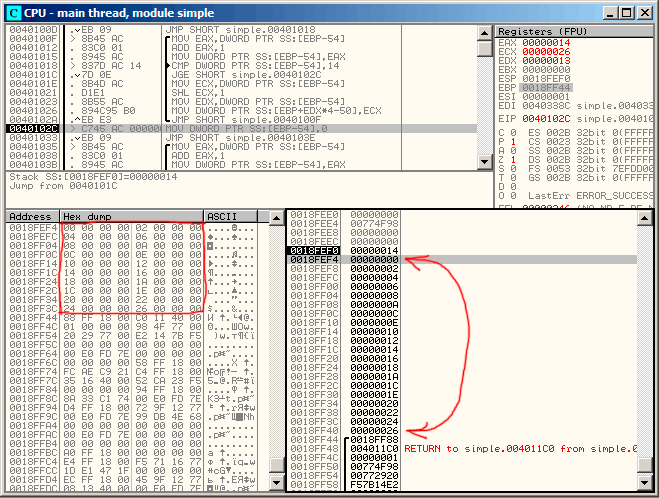
\includegraphics[scale=\FigScale]{patterns/13_arrays/1_simple/olly.png}
\caption{\olly: \RU{после заполнения массива}\EN{after array filling}}
\label{fig:array_simple_olly}
\end{figure}

\RU{А так как этот массив находится в стеке, то мы видим все его 20 элементов внутри стека.}
\EN{Since this array is located in stack, we see all its 20 elements inside of stack.}

\fi

\subsubsection{GCC}

\RU{То, что делает GCC 4.4.1:}\EN{Here is what GCC 4.4.1 does:}

\lstinputlisting[caption=GCC 4.4.1]{patterns/13_arrays/1_simple/simple_gcc.asm}

\RU{Кстати, переменная $a$ в нашем примере имеет тип \IT{int*} (то есть, указатель на \Tint{}) ~--- вы можете попробовать передать в другую функцию указатель на массив, но точнее было бы сказать, что передается указатель на первый элемент массива (а адреса остальных элементов массива можно вычислить очевидным образом).}\EN{By the way, $a$ variable has \IT{int*} type 
(the pointer to \Tint{})~---you can try to pass a pointer to array to another function, but it much correctly to say the pointer to the first array element is passed (addresses of another element's places are calculated in obvious way).}
\RU{Если индексировать этот указатель как \IT{a[idx]}, \IT{idx} просто прибавляется к указателю и возвращается элемент, расположенный там, куда ссылается вычисленный указатель.}\EN{If to index this pointer as \IT{a[idx]}, \IT{idx} just to be added to the pointer and the element placed there (to which calculated pointer is pointing) returned.}

\RU{Вот любопытный пример: строка символов вроде \IT{``string''} это массив из символов, 
и она имеет тип \IT{const char[]}.}\EN{An interesting example: string of characters like 
\IT{``string''} is array of characters and it has \IT{const char[]} type.}
\RU{К этому указателю также можно применять индекc.}
\EN{Index can also be applied to this pointer.}
\RU{И поэтому можно написать даже так:  \TT{``string''[i]} ~--- это совершенно легальное выражение в \CCpp!}
\EN{And that is why it is possible to write like \TT{``string''[i]}~---this is correct \CCpp expression!}

\ifdefined\IncludeARM
\subsection{ARM}

\subsubsection{\NonOptimizingKeilVI (\ARMMode)}

\lstinputlisting{patterns/13_arrays/1_simple/simple_Keil_ARM_O0.asm.\LANG}

\RU{Тип \Tint требует 32 бита для хранения (или 4 байта),}
\EN{\Tint type requires 32 bits for storage (or 4 bytes),}
\RU{так что для хранения 20 переменных типа \Tint, нужно $80$ (\TT{0x50}) байт.}
\EN{so to store 20 \Tint variables $80$ (\TT{0x50}) bytes are needed.}
\RU{Поэтому инструкция}\EN{So that is why the} \TT{\q{SUB SP, SP, \#0x50}} 
\RU{в прологе функции выделяет в локальном стеке под массив именно столько места.}
\EN{instruction in the function's prologie allocates exactly this amount of space in the stack.}

\RU{И в первом и во втором цикле, итератор цикла $i$ будет постоянно находится в регистре \Reg{4}.}
\EN{In both the first and second loops, the loop iterator $i$ is placed in the \Reg{4} register.}

\index{ARM!Optional operators!LSL}
\RU{Число, которое нужно записать в массив, вычисляется так: $i*2$, и это эквивалентно 
сдвигу на 1 бит влево, так что инструкция \TT{\q{MOV R0, R4,LSL\#1}} делает это.}
\EN{The number that is to be written into the array is calculated as $i*2$, which is effectively equivalent 
to shifting it left by one bit, so \TT{\q{MOV R0, R4,LSL\#1}} instruction does this.}

\index{ARM!\Instructions!STR}
\TT{\q{STR R0, [SP,R4,LSL\#2]}} \RU{записывает содержимое \Reg{0} в массив}\EN{writes the contents of \Reg{0} into the array}.
\RU{Указатель на элемент массива вычисляется так: \ac{SP} указывает на начало массива, \Reg{4} это $i$.}
\EN{Here is how a pointer to array element is calculated: \ac{SP} points to the start of the array, \Reg{4} is $i$.}
\RU{Так что сдвигаем $i$ на 2 бита влево, что эквивалентно умножению на $4$ 
(ведь каждый элемент массива занимает 4 байта) и прибавляем это к адресу начала массива.}
\EN{So shifting $i$ left by 2 bits is effectively equivalent to multiplication by $4$
(since each array element has a size of 4 bytes) and then it's added to the address of the start of the array.}

\index{ARM!\Instructions!LDR}
\RU{Во втором цикле используется обратная инструкция \TT{\q{LDR R2, [SP,R4,LSL\#2]}},
она загружает из массива нужное значение, и указатель на него вычисляется точно так же.}
\EN{The second loop has an inverse \TT{\q{LDR R2, [SP,R4,LSL\#2]}}
instruction, it loads the value we need from the array, and the pointer to it is calculated likewise.}

\subsubsection{\OptimizingKeilVI (\ThumbMode)}

\lstinputlisting{patterns/13_arrays/1_simple/simple_Keil_thumb_O3.asm.\LANG}

\RU{Код для thumb очень похожий.}\EN{Thumb code is very similar.}
\index{ARM!\Instructions!LSLS}
\RU{В thumb имеются отдельные инструкции для битовых сдвигов (как \TT{LSLS}), 
вычисляющие и число для записи в массив и адрес каждого элемента массива.}
\EN{Thumb mode has special instructions for bit shifting (like \TT{LSLS}),
which calculates the value to be written into the array and the address of each element in the array as well.}

\RU{Компилятор почему-то выделил в локальном стеке немного больше места, 
однако последние 4 байта не используются.}
\EN{The compiler allocates slightly more space in the local stack, however, the last 4 bytes are not used.}

\subsubsection{\NonOptimizing GCC 4.9.1 (ARM64)}

\lstinputlisting[caption=\NonOptimizing GCC 4.9.1 (ARM64)]{patterns/13_arrays/1_simple/ARM64_GCC491_O0.s.\LANG}

\fi

\section{\RU{Переполнение буфера}\EN{Buffer overflow}}
\label{subsec:bufferoverflow}
\myindex{\BufferOverflow}

\EN{\subsection{Reading outside array bounds}

So, array indexing is just \IT{array\lbrack{}index\rbrack}.
If you study the generated code closely, you'll probably note the missing index bounds checking,
which could check \IT{if it is less than 20}.
What if the index is 20 or greater?
That's the one \CCpp feature it is often blamed for.

Here is a code that successfully compiles and works:

\lstinputlisting{patterns/13_arrays/2_BO/r.c}

Compilation results (MSVC 2008):

\lstinputlisting[caption=\NonOptimizing MSVC 2008]{patterns/13_arrays/2_BO/r_msvc.asm}

The code produced this result:

\begin{figure}[h]
\centering
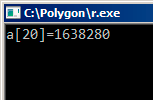
\includegraphics[scale=\NormalScale]{patterns/13_arrays/2_BO/olly_r3.png}
\caption{\olly: console output}
\label{fig:array_BO_olly_r3}
\end{figure}

It is just \IT{something} that was lying in the stack near to the array, 80 bytes away from its first element.

\clearpage
\myindex{\olly}
Let's try to find out where did this value come from, using \olly.

Let's load and find the value located right after the last array element:

\begin{figure}[H]
\centering
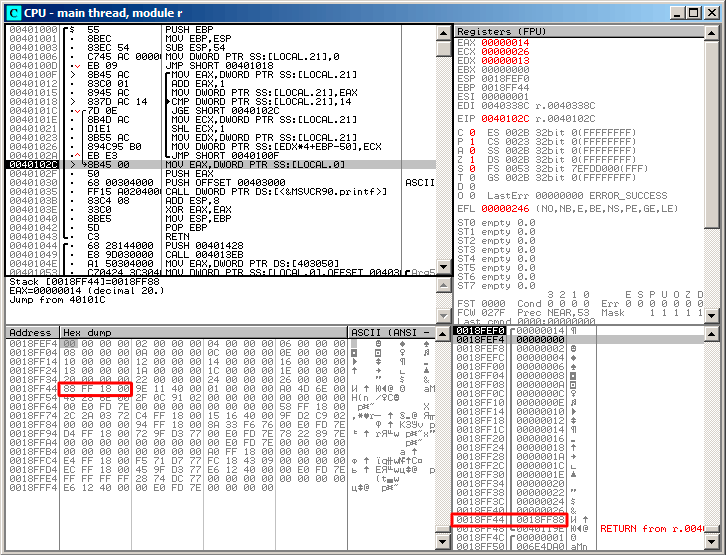
\includegraphics[scale=\FigScale]{patterns/13_arrays/2_BO/olly_r1.png}
\caption{\olly: reading of the 20th element and execution of \printf}
\label{fig:array_BO_olly_r1}
\end{figure}

What is this? 
Judging by the stack layout,
this is the saved value of the EBP register.
\clearpage
Let's trace further and see how it gets restored:

\begin{figure}[H]
\centering
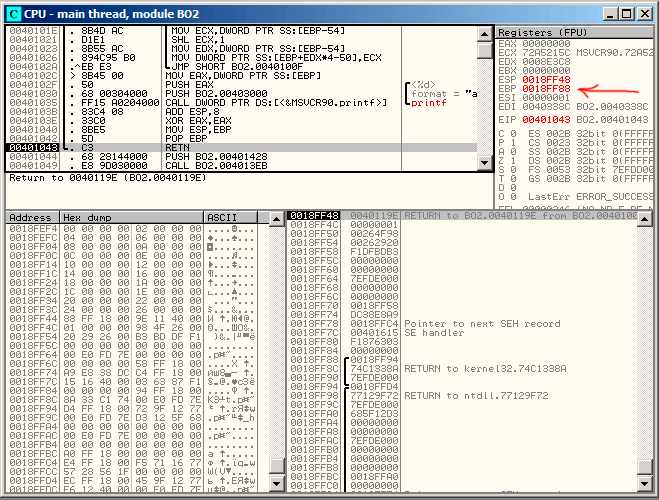
\includegraphics[scale=\FigScale]{patterns/13_arrays/2_BO/olly_r2.png}
\caption{\olly: restoring value of EBP}
\label{fig:array_BO_olly_r2}
\end{figure}

Indeed, how it could be different?
The compiler may generate some additional code to check the index value to be always
in the array's bounds (like in higher-level programming languages\footnote{Java, Python, etc})
but this makes the code slower.

}
\RU{\subsectionold{Чтение за пределами массива}

Итак, индексация массива --- это просто \IT{массив\lbrack{}индекс\rbrack}.  % TODO1 как-то плохо отображаются []
Если вы присмотритесь к коду, в цикле печати значений массива через \printf вы 
не увидите проверок индекса, \IT{меньше ли он двадцати?} 
А что будет если он будет 20 или больше? 
Эта одна из особенностей \CCpp, за которую их, собственно, и ругают.

Вот код, который и компилируется и работает:

\lstinputlisting{patterns/13_arrays/2_BO/r.c}

Вот результат компиляции в (MSVC 2008):

\lstinputlisting[caption=\NonOptimizing MSVC 2008]{patterns/13_arrays/2_BO/r_msvc.asm}

Данный код при запуске выдал вот такой результат:

\begin{figure}[h]
\centering
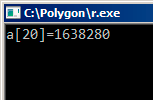
\includegraphics[scale=\NormalScale]{patterns/13_arrays/2_BO/olly_r3.png}
\caption{\olly: вывод в консоль}
\label{fig:array_BO_olly_r3}
\end{figure}

Это просто \IT{что-то}, что волею случая лежало в стеке рядом с массивом, 
через 80 байт от его первого элемента.

\clearpage
\myindex{\olly}
Попробуем узнать в \olly, что это за значение.
Загружаем и находим это значение, находящееся точно после последнего элемента массива:

\begin{figure}[H]
\centering
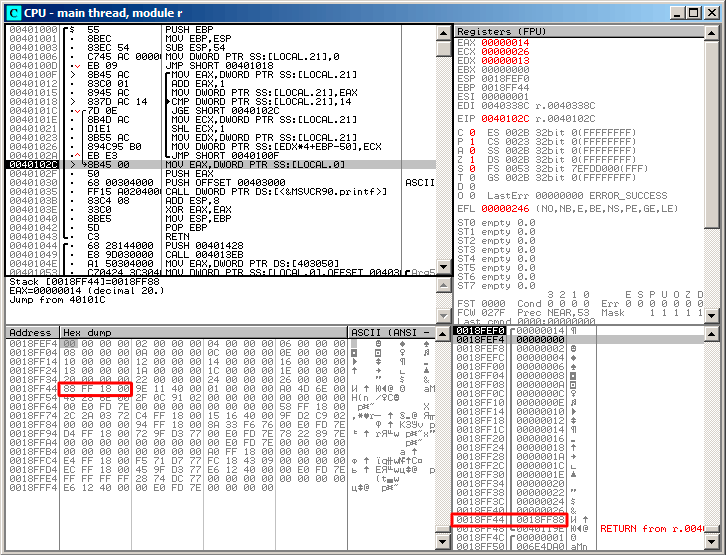
\includegraphics[scale=\FigScale]{patterns/13_arrays/2_BO/olly_r1.png}
\caption{\olly: чтение 20-го элемента и вызов \printf}
\label{fig:array_BO_olly_r1}
\end{figure}

Что это за значение? 
Судя по разметке стека, это сохраненное значение регистра EBP.
\clearpage
Трассируем далее, и видим, как оно восстанавливается:

\begin{figure}[H]
\centering
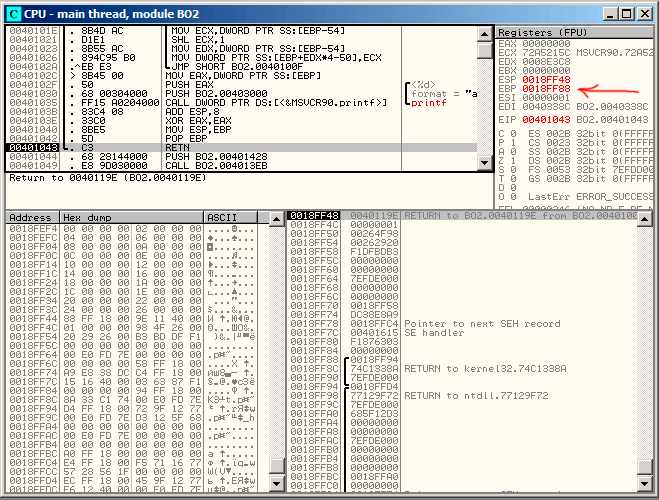
\includegraphics[scale=\FigScale]{patterns/13_arrays/2_BO/olly_r2.png}
\caption{\olly: восстановление EBP}
\label{fig:array_BO_olly_r2}
\end{figure}

Действительно, а как могло бы быть иначе? Компилятор мог бы встроить какой-то код, 
каждый раз проверяющий индекс на соответствие пределам массива, как в языках программирования 
более высокого уровня\footnote{Java, Python, итд.}, что делало бы запускаемый код медленнее.

}
\EN{\subsubsection{Writing beyond array bounds}

OK, we read some values from the stack \IT{illegally}, but what if we could write something to it?

Here is what we have got:

\lstinputlisting{patterns/13_arrays/2_BO/w.c}

\myparagraph{MSVC}

And what we get:

\lstinputlisting[caption=\NonOptimizing MSVC 2008]{patterns/13_arrays/2_BO/w_EN.asm}

The compiled program crashes after running. No wonder. Let's see where exactly does it is crash.

\clearpage
\myindex{\olly}

Let's load it into \olly, and trace until all 30 elements are written:

\begin{figure}[H]
\centering
\myincludegraphics{patterns/13_arrays/2_BO/olly_w1.png}
\caption{\olly: after restoring the value of EBP}
\label{fig:array_BO_olly_w1}
\end{figure}

\clearpage
Trace until the function end:

\begin{figure}[H]
\centering
\myincludegraphics{patterns/13_arrays/2_BO/olly_w2.png}
\caption{\olly: 
EIP was restored, but \olly can't disassemble at 0x15}
\label{fig:array_BO_olly_w2}
\end{figure}

Now please keep your eyes on the registers.

\EIP is 0x15 now. It is not a legal address for code---at least for win32 code!
We got there somehow against our will.
It is also interesting that the \EBP register contain 0x14,
\ECX and \EDX contain 0x1D.

Let's study stack layout a bit more.

After the control flow was passed to \TT{\main}, the value in the \EBP register was saved on the stack.
Then, 84 bytes were allocated for the array and the $i$ variable.
That's \TT{(20+1)*sizeof(int)}.
\ESP now points to the \TT{\_i} variable in the local stack and after the execution of 
the next \TT{PUSH something}, \IT{something} is appearing next to \TT{\_i}.

That's the stack layout while the control is in \main:

\begin{center}
\begin{tabular}{ | l | l | }
\hline
  \TT{ESP}    & 4 bytes allocated for $i$ variable \\
\hline
  \TT{ESP+4}  & 80 bytes allocated for \TT{a[20]} array \\
\hline
  \TT{ESP+84} & saved \EBP value \\
\hline
  \TT{ESP+88} & return address \\
\hline
\end{tabular}
\end{center}

\TT{a[19]=something} statement writes the last \Tint in the bounds of the array (in bounds so far!).

\TT{a[20]=something} statement writes \IT{something} to the place where the value of \EBP is saved.

Please take a look at the register state at the moment of the crash. In our case,
20 was written in the 20th element. 
At the function end, the function epilogue restores the original \EBP value.
(20 in decimal is \TT{0x14} in hexadecimal).
Then \RET gets executed, which is effectively equivalent to \TT{POP EIP} instruction.

The \RET instruction takes the return address from the stack (that is the address in \ac{CRT}),
which was called \main),
and 21 iss stored there (\TT{0x15} in hexadecimal).
The CPU traps at address \TT{0x15},
but there is no executable code there, so exception gets raised.

\myindex{\BufferOverflow}

Welcome! It is called a \IT{buffer overflow}\footnote{\href{http://go.yurichev.com/17132}{wikipedia}}.

Replace the \Tint array with a string (\Tchar array), create a long string deliberately
and pass it to the program, to the function, which doesn't check the length of the string and copies it in a short buffer,
and you'll able to point the program to an address to which it must jump.
It's not that simple in reality, but that is how it emerged.
Classic article about it: \AlephOne.

\myparagraph{GCC}

Let's try the same code in GCC 4.4.1. We get:

\lstinputlisting{patterns/13_arrays/2_BO/w_gcc.asm}

Running this in Linux will produce: \TT{Segmentation fault}.

\myindex{GDB}

If we run this in the GDB debugger, we get this:

\begin{lstlisting}
(gdb) r
Starting program: /home/dennis/RE/1 

Program received signal SIGSEGV, Segmentation fault.
0x00000016 in ?? ()
(gdb) info registers
eax            0x0	0
ecx            0xd2f96388	-755407992
edx            0x1d	29
ebx            0x26eff4	2551796
esp            0xbffff4b0	0xbffff4b0
ebp            0x15	0x15
esi            0x0	0
edi            0x0	0
eip            0x16	0x16
eflags         0x10202	[ IF RF ]
cs             0x73	115
ss             0x7b	123
ds             0x7b	123
es             0x7b	123
fs             0x0	0
gs             0x33	51
(gdb) 
\end{lstlisting}

The register values are slightly different than in win32 example, 
since the stack layout is slightly different too.

}
\RU{\subsectionold{Запись за пределы массива}

Итак, мы прочитали какое-то число из стека явно \IT{нелегально}, а что если мы запишем?

Вот что мы пишем:

\lstinputlisting{patterns/13_arrays/2_BO/w.c}

\subsubsectionold{MSVC}

И вот что имеем на ассемблере:

\lstinputlisting[caption=\NonOptimizing MSVC 2008]{patterns/13_arrays/2_BO/w_RU.asm}

Запускаете скомпилированную программу, и она падает. Немудрено. Но давайте теперь узнаем, где именно.

\clearpage
\myindex{\olly}

Загружаем в \olly, трассируем пока запишутся все 30 элементов:

\begin{figure}[H]
\centering
\myincludegraphics{patterns/13_arrays/2_BO/olly_w1.png}
\caption{\olly: после восстановления EBP}
\label{fig:array_BO_olly_w1}
\end{figure}

\clearpage
Доходим до конца функции:

\begin{figure}[H]
\centering
\myincludegraphics{patterns/13_arrays/2_BO/olly_w2.png}
\caption{\olly: EIP восстановлен, но \olly не может дизассемблировать по адресу 0x15}
\label{fig:array_BO_olly_w2}
\end{figure}

Итак, следите внимательно за регистрами.

\EIP теперь 0x15. Это явно нелегальный адрес для кода~--- по крайней мере, win32-кода! 
Мы там как-то очутились, причем, сами того не хотели. Интересен также тот факт, что в \EBP хранится 0x14, 
а в \ECX и \EDX хранится 0x1D.

Ещё немного изучим разметку стека.

После того как управление передалось в \main, в стек было сохранено значение \EBP. 
Затем для массива и переменной $i$ было выделено 84 байта. Это \TT{(20+1)*sizeof(int)}. 
\ESP сейчас указывает на переменную \TT{\_i} в локальном стеке и при исполнении следующего \INS{PUSH что-либо}, 
\IT{что-либо} появится рядом с \TT{\_i}.

Вот так выглядит разметка стека пока управление находится внутри \main:

\begin{center}
\begin{tabular}{ | l | l | }
\hline
  \TT{ESP}    & 4 байта выделенных для переменной $i$ \\
\hline
  \TT{ESP+4}  & 80 байт выделенных для массива \TT{a[20]} \\
\hline
  \TT{ESP+84} & сохраненное значение \EBP \\
\hline
  \TT{ESP+88} & адрес возврата \\
\hline
\end{tabular}
\end{center}

Выражение \TT{a[19]=что\_нибудь} записывает последний \Tint в пределах массива (пока что в пределах!).

Выражение \TT{a[20]=что\_нибудь} записывает \IT{что\_нибудь} на место где сохранено значение \EBP.

Обратите внимание на состояние регистров на момент падения процесса. В нашем случае 
в 20-й элемент записалось значение 20. 
И вот всё дело в том, что заканчиваясь, эпилог функции восстанавливал значение \EBP 
(20 в десятичной системе это как раз \TT{0x14} в шестнадцатеричной). 
Далее выполнилась инструкция \RET, которая на самом деле эквивалентна \TT{POP EIP}.

Инструкция \RET вытащила из стека адрес возврата (это адрес где-то внутри \ac{CRT}), которая вызвала \main),
а там было записано 21 в десятичной системе, то есть 0x15 в шестнадцатеричной. 
И вот процессор оказался по адресу 0x15, но исполняемого кода там нет, так что случилось исключение.

\myindex{\BufferOverflow}
Добро пожаловать! Это называется \IT{buffer overflow}\footnote{\href{http://go.yurichev.com/17132}{wikipedia}}.

Замените массив \Tint на строку (массив \Tchar), нарочно создайте слишком длинную строку, 
передайте её в ту программу, 
в ту функцию, которая не проверяя длину строки скопирует её в слишком короткий буфер, 
и вы сможете указать программе, по какому именно адресу перейти. 
Не всё так просто в реальности, конечно, но началось всё с этого.
Классическая статья об этом: \AlephOne.

\subsubsectionold{GCC}

Попробуем то же самое в GCC 4.4.1. У нас выходит такое:

\lstinputlisting{patterns/13_arrays/2_BO/w_gcc.asm}

Запуск этого в Linux выдаст: \TT{Segmentation fault}.

\myindex{GDB}
Если запустить полученное в отладчике GDB, получим:

\begin{lstlisting}
(gdb) r
Starting program: /home/dennis/RE/1 

Program received signal SIGSEGV, Segmentation fault.
0x00000016 in ?? ()
(gdb) info registers
eax            0x0	0
ecx            0xd2f96388	-755407992
edx            0x1d	29
ebx            0x26eff4	2551796
esp            0xbffff4b0	0xbffff4b0
ebp            0x15	0x15
esi            0x0	0
edi            0x0	0
eip            0x16	0x16
eflags         0x10202	[ IF RF ]
cs             0x73	115
ss             0x7b	123
ds             0x7b	123
es             0x7b	123
fs             0x0	0
gs             0x33	51
(gdb) 
\end{lstlisting}

Значения регистров немного другие, чем в примере win32, потому что разметка стека чуть другая.

}


\EN{\subsection{Buffer overflow protection methods}
\label{subsec:BO_protection}

There are several methods to protect against this scourge, regardless of the \CCpp programmers' negligence.
MSVC has options like\footnote{compiler-side buffer overflow protection methods:
\href{http://go.yurichev.com/17133}{wikipedia.org/wiki/Buffer\_overflow\_protection}}:

\begin{lstlisting}
 /RTCs Stack Frame runtime checking
 /GZ Enable stack checks (/RTCs)
\end{lstlisting}

\myindex{x86!\Instructions!RET}
\myindex{Function prologue}
\myindex{Security cookie}

One of the methods is to write a random value between the local variables in stack at function prologue 
and to check it in function epilogue before the function exits.
If value is not the same, do not execute the last instruction \RET, but stop (or hang).
The process will halt, but that is much better than a remote attack to your host.
    
\newcommand{\CANARYURL}{\href{http://go.yurichev.com/17134}{wikipedia.org/wiki/Domestic\_canary\#Miner.27s\_canary}}

\myindex{Canary}

This random value is called a \q{canary} sometimes, it is related to the miners' canary\footnote{\CANARYURL},
they were used by miners in the past days in order to detect poisonous gases quickly.

Canaries are very sensitive to mine gases, they become very agitated in case of danger, or even die.

If we compile our very simple array example~(\myref{arrays_simple}) in \ac{MSVC}
with RTC1 and RTCs option,\\
you can see a call to \TT{@\_RTC\_CheckStackVars@8} a function at the end of the function that checks if the \q{canary} is correct.

Let's see how GCC handles this. 
Let's take an \TT{alloca()}~(\myref{alloca}) example:

\lstinputlisting{patterns/02_stack/04_alloca/2_1.c}

By default, without any additional options, GCC 4.7.3 inserts a \q{canary} check into the code:

\lstinputlisting[caption=GCC 4.7.3]{patterns/13_arrays/3_BO_protection/gcc_canary_EN.asm}

\myindex{x86!\Registers!GS}
The random value is located in \TT{gs:20}. 
It gets written on the stack and then at the end of the function
the value in the stack is compared with the correct \q{canary} in \TT{gs:20}. 
If the values are not equal, the 
\TT{\_\_stack\_chk\_fail} 
function is called and we can see in the console something like that (Ubuntu 13.04 x86):

\begin{lstlisting}
*** buffer overflow detected ***: ./2_1 terminated
======= Backtrace: =========
/lib/i386-linux-gnu/libc.so.6(__fortify_fail+0x63)[0xb7699bc3]
/lib/i386-linux-gnu/libc.so.6(+0x10593a)[0xb769893a]
/lib/i386-linux-gnu/libc.so.6(+0x105008)[0xb7698008]
/lib/i386-linux-gnu/libc.so.6(_IO_default_xsputn+0x8c)[0xb7606e5c]
/lib/i386-linux-gnu/libc.so.6(_IO_vfprintf+0x165)[0xb75d7a45]
/lib/i386-linux-gnu/libc.so.6(__vsprintf_chk+0xc9)[0xb76980d9]
/lib/i386-linux-gnu/libc.so.6(__sprintf_chk+0x2f)[0xb7697fef]
./2_1[0x8048404]
/lib/i386-linux-gnu/libc.so.6(__libc_start_main+0xf5)[0xb75ac935]
======= Memory map: ========
08048000-08049000 r-xp 00000000 08:01 2097586    /home/dennis/2_1
08049000-0804a000 r--p 00000000 08:01 2097586    /home/dennis/2_1
0804a000-0804b000 rw-p 00001000 08:01 2097586    /home/dennis/2_1
094d1000-094f2000 rw-p 00000000 00:00 0          [heap]
b7560000-b757b000 r-xp 00000000 08:01 1048602    /lib/i386-linux-gnu/libgcc_s.so.1
b757b000-b757c000 r--p 0001a000 08:01 1048602    /lib/i386-linux-gnu/libgcc_s.so.1
b757c000-b757d000 rw-p 0001b000 08:01 1048602    /lib/i386-linux-gnu/libgcc_s.so.1
b7592000-b7593000 rw-p 00000000 00:00 0
b7593000-b7740000 r-xp 00000000 08:01 1050781    /lib/i386-linux-gnu/libc-2.17.so
b7740000-b7742000 r--p 001ad000 08:01 1050781    /lib/i386-linux-gnu/libc-2.17.so
b7742000-b7743000 rw-p 001af000 08:01 1050781    /lib/i386-linux-gnu/libc-2.17.so
b7743000-b7746000 rw-p 00000000 00:00 0
b775a000-b775d000 rw-p 00000000 00:00 0
b775d000-b775e000 r-xp 00000000 00:00 0          [vdso]
b775e000-b777e000 r-xp 00000000 08:01 1050794    /lib/i386-linux-gnu/ld-2.17.so
b777e000-b777f000 r--p 0001f000 08:01 1050794    /lib/i386-linux-gnu/ld-2.17.so
b777f000-b7780000 rw-p 00020000 08:01 1050794    /lib/i386-linux-gnu/ld-2.17.so
bff35000-bff56000 rw-p 00000000 00:00 0          [stack]
Aborted (core dumped)
\end{lstlisting}

\myindex{MS-DOS}
gs is the so-called segment register. These registers were used widely in MS-DOS and DOS-extenders
times.
Today, its function is different.
\myindex{TLS}
\myindex{Windows!TIB}

To say it briefly, the \TT{gs} register in Linux always points to the
\ac{TLS}~(\myref{TLS})---some information specific to thread is stored there.
By the way, in win32 the \TT{fs} register plays the same role, pointing to
\ac{TIB} \footnote{\href{http://go.yurichev.com/17104}{wikipedia.org/wiki/Win32\_Thread\_Information\_Block}}. 

More information can be found in the Linux kernel source code (at least in 3.11 version),\\
in \IT{arch/x86/include/asm/stackprotector.h} this variable is described in the comments.

\subsectionold{\OptimizingXcodeIV (\ThumbTwoMode)}


Let's get back to our simple array example (\myref{arrays_simple}),

again, now we can see how LLVM checks the correctness of the \q{canary}:

% TODO shorten the listing a bit? is full display of unrolled loop necessary?
\lstinputlisting{patterns/13_arrays/3_BO_protection/simple_Xcode_thumb_O3_EN.asm}

\myindex{Unrolled loop}

First of all, as we see, LLVM \q{unrolled} the loop and all values were written into an array one-by-one,
pre-calculated, as LLVM concluded it can work faster.
By the way, instructions in ARM mode may help to do this even faster, 
and finding this could be your homework.


At the function end we see the comparison of the \q{canaries}---the one in the local stack and the correct one,
to which \Reg{8} points.
\myindex{ARM!\Instructions!IT}

If they are equal to each other, a 4-instruction block is triggered by \INS{ITTTT EQ},
which contains writing 0 in \Reg{0}, the function epilogue and exit.
If the \q{canaries} are not equal, the block being skipped,
and the jump to \TT{\_\_\_stack\_chk\_fail}
 function will occur, which, perhaps will halt execution.
% TODO1 illustrate this!


}
\RU{\section{Защита от переполнения буфера}
\label{subsec:BO_protection}

В наше время пытаются бороться с переполнением буфера невзирая на халатность программистов на \CCpp. 
В MSVC есть опции вроде\footnote{описания защит, которые компилятор может вставлять в код:
\href{http://go.yurichev.com/17133}{wikipedia.org/wiki/Buffer\_overflow\_protection}}:

\begin{lstlisting}
 /RTCs Stack Frame runtime checking
 /GZ Enable stack checks (/RTCs)
\end{lstlisting}

\myindex{x86!\Instructions!RET}
\myindex{Function prologue}
\myindex{Security cookie}
Одним из методов является вставка в прологе функции некоего случайного значения в область локальных переменных 
и проверка этого значения в эпилоге функции перед выходом. 
Если проверка не прошла, то не выполнять инструкцию \RET, а остановиться (или зависнуть). 
Процесс зависнет, но это лучше, чем удаленная атака на ваш компьютер.

\newcommand{\CANARYURL}{\href{http://go.yurichev.com/17135}{miningwiki.ru/wiki/Канарейка\_в\_шахте}}

\myindex{Canary}
Это случайное значение иногда называют \q{канарейкой}
\footnote{\q{canary} в англоязычной литературе}, 
по аналогии с шахтной канарейкой\footnote{\CANARYURL}.
Раньше использовали шахтеры, чтобы определять, есть ли в шахте опасный газ.

Канарейки очень к нему чувствительны и либо проявляли сильное беспокойство, либо гибли от газа.

Если скомпилировать наш простейший пример работы с массивом ~(\myref{arrays_simple}) в \ac{MSVC}
с опцией RTC1 или RTCs, в конце нашей функции будет вызов функции
\TT{@\_RTC\_CheckStackVars@8}, проверяющей корректность \q{канарейки}.

Посмотрим, как дела обстоят в GCC. 
Возьмем пример из секции про \TT{alloca()}~(\myref{alloca}):

\lstinputlisting{patterns/02_stack/04_alloca/2_1.c}

По умолчанию, без дополнительных ключей, GCC 4.7.3 вставит в код проверку \q{канарейки}:

\lstinputlisting[caption=GCC 4.7.3]{patterns/13_arrays/3_BO_protection/gcc_canary_RU.asm}

\myindex{x86!\Registers!GS}
Случайное значение находится в \TT{gs:20}. 
Оно записывается в стек, затем, в конце функции, значение в стеке
сравнивается с корректной \q{канарейкой} в \TT{gs:20}. 
Если значения не равны, будет вызвана функция 
\TT{\_\_stack\_chk\_fail} и в консоли мы увидим что-то вроде такого
 (Ubuntu 13.04 x86):

\begin{lstlisting}
*** buffer overflow detected ***: ./2_1 terminated
======= Backtrace: =========
/lib/i386-linux-gnu/libc.so.6(__fortify_fail+0x63)[0xb7699bc3]
/lib/i386-linux-gnu/libc.so.6(+0x10593a)[0xb769893a]
/lib/i386-linux-gnu/libc.so.6(+0x105008)[0xb7698008]
/lib/i386-linux-gnu/libc.so.6(_IO_default_xsputn+0x8c)[0xb7606e5c]
/lib/i386-linux-gnu/libc.so.6(_IO_vfprintf+0x165)[0xb75d7a45]
/lib/i386-linux-gnu/libc.so.6(__vsprintf_chk+0xc9)[0xb76980d9]
/lib/i386-linux-gnu/libc.so.6(__sprintf_chk+0x2f)[0xb7697fef]
./2_1[0x8048404]
/lib/i386-linux-gnu/libc.so.6(__libc_start_main+0xf5)[0xb75ac935]
======= Memory map: ========
08048000-08049000 r-xp 00000000 08:01 2097586    /home/dennis/2_1
08049000-0804a000 r--p 00000000 08:01 2097586    /home/dennis/2_1
0804a000-0804b000 rw-p 00001000 08:01 2097586    /home/dennis/2_1
094d1000-094f2000 rw-p 00000000 00:00 0          [heap]
b7560000-b757b000 r-xp 00000000 08:01 1048602    /lib/i386-linux-gnu/libgcc_s.so.1
b757b000-b757c000 r--p 0001a000 08:01 1048602    /lib/i386-linux-gnu/libgcc_s.so.1
b757c000-b757d000 rw-p 0001b000 08:01 1048602    /lib/i386-linux-gnu/libgcc_s.so.1
b7592000-b7593000 rw-p 00000000 00:00 0
b7593000-b7740000 r-xp 00000000 08:01 1050781    /lib/i386-linux-gnu/libc-2.17.so
b7740000-b7742000 r--p 001ad000 08:01 1050781    /lib/i386-linux-gnu/libc-2.17.so
b7742000-b7743000 rw-p 001af000 08:01 1050781    /lib/i386-linux-gnu/libc-2.17.so
b7743000-b7746000 rw-p 00000000 00:00 0
b775a000-b775d000 rw-p 00000000 00:00 0
b775d000-b775e000 r-xp 00000000 00:00 0          [vdso]
b775e000-b777e000 r-xp 00000000 08:01 1050794    /lib/i386-linux-gnu/ld-2.17.so
b777e000-b777f000 r--p 0001f000 08:01 1050794    /lib/i386-linux-gnu/ld-2.17.so
b777f000-b7780000 rw-p 00020000 08:01 1050794    /lib/i386-linux-gnu/ld-2.17.so
bff35000-bff56000 rw-p 00000000 00:00 0          [stack]
Aborted (core dumped)
\end{lstlisting}

\myindex{MS-DOS}
gs это так называемый сегментный регистр. Эти регистры широко использовались во времена MS-DOS 
и DOS-экстендеров.
Сейчас их функция немного изменилась.
\myindex{TLS}
\myindex{Windows!TIB}
Если говорить кратко, в Linux \TT{gs} всегда указывает на \ac{TLS}~(\myref{TLS})~--- там находится различная 
информация, специфичная для выполняющегося потока.

Кстати, в win32 эту же роль играет сегментный регистр \TT{fs},
он всегда указывает на
\ac{TIB} \footnote{\href{http://go.yurichev.com/17104}{wikipedia.org/wiki/Win32\_Thread\_Information\_Block}}. 

Больше информации можно почерпнуть из исходных кодов Linux (по крайней мере, в версии 3.11): 
в файле \IT{arch/x86/include/asm/stackprotector.h} в комментариях описывается эта переменная.

\subsectionold{\OptimizingXcodeIV (\ThumbTwoMode)}

Возвращаясь к нашему простому примеру
 (\myref{arrays_simple}),
можно посмотреть, как LLVM добавит проверку \q{канарейки}:

% TODO shorten the listing a bit? is full display of unrolled loop necessary?
\lstinputlisting{patterns/13_arrays/3_BO_protection/simple_Xcode_thumb_O3_RU.asm}

\myindex{Unrolled loop}
Во-первых, LLVM \q{развернул} цикл и все значения записываются в массив по одному, 
уже вычисленные, потому что LLVM посчитал что так будет быстрее.

Кстати, инструкции режима ARM позволяют сделать это ещё быстрее и это может быть вашим 
домашним заданием.

В конце функции мы видим сравнение \q{канареек}~--- той что лежит в локальном стеке и корректной, 
на которую ссылается регистр \Reg{8}.

\myindex{ARM!\Instructions!IT}
Если они равны, срабатывает блок из четырех инструкций при помощи \INS{ITTTT EQ}.
Это запись 0 в \Reg{0}, эпилог функции и выход из нее.

Если \q{канарейки} не равны, блок не срабатывает и происходит
переход на функцию \TT{\_\_\_stack\_chk\_fail}, которая, вероятно, остановит работу программы.

% TODO1 illustrate this!

}
\subsection{\RU{Еще немного о массивах}\EN{One more word about arrays}}

\RU{Теперь понятно, почему нельзя написать в исходном коде на \CCpp что-то вроде:}
\EN{Now we understand why it is impossible to write something like this in \CCpp code:}

\begin{lstlisting}
void f(int size)
{
    int a[size];
...
};
\end{lstlisting}

\RU{Чтобы выделить место под массив в локальном стеке, 
компилятору нужно знать размер массива, чего он на стадии компиляции, 
разумеется, знать не может.}
\EN{That's just because the compiler must know the exact array size to allocate space for 
it in the local stack layout on at the compiling stage.}

\myindex{\CLanguageElements!C99!variable length arrays}
\myindex{\CStandardLibrary!alloca()}
\RU{Если вам нужен массив произвольной длины, то выделите столько, сколько нужно, через \TT{malloc()}, 
а затем обращайтесь к выделенному блоку байт как к массиву того типа, который вам нужен.}
\EN{If you need an array of arbitrary size, allocate it by using \TT{malloc()}, then access the allocated memory block
as an array of variables of the type you need.}

\RU{Либо используйте возможность стандарта C99~ \InSqBrackets{\CNineNineStd 6.7.5/2},
и внутри это очень похоже на \IT{alloca()}~(\myref{alloca}).}
\EN{Or use the C99 standard feature \InSqBrackets{\CNineNineStd 6.7.5/2},
and it works like \IT{alloca()}~(\myref{alloca}) internally.}

\RU{Для работы в с памятью, можно также воспользоваться библиотекой сборщика мусора в Си.}
\EN{It's also possible to use garbage collecting libraries for C.}
\RU{А для языка Си++ есть библиотеки с поддержкой умных указателей.}
\EN{And there are also libraries supporting smart pointers for C++.}


\EN{\subsection{Array of pointers to strings}
\label{array_of_pointers_to_strings}

Here is an example for an array of pointers.

\lstinputlisting[caption=Get month name,label=get_month1]{patterns/13_arrays/45_month_1D/month1_EN.c}

\subsubsection{x64}

\lstinputlisting[caption=\Optimizing MSVC 2013 x64]{patterns/13_arrays/45_month_1D/month1_MSVC_2013_x64_Ox.asm}

The code is very simple:

\begin{itemize}

\item
\myindex{x86!\Instructions!MOVSXD}

The first \INS{MOVSXD} instruction copies a 32-bit value from \ECX (where $month$ argument is passed) 
to \RAX with sign-extension (because the $month$ argument is of type \Tint).

The reason for the sign extension is that this 32-bit value is to be used in calculations
with other 64-bit values.

Hence, it has to be promoted to 64-bit%
\footnote{It is somewhat weird, but negative array index could be passed here as $month$
(negative array indices will have been explained later: \myref{negative_array_indices}).
And if this happens, the negative input value of \Tint type is sign-extended correctly 
and the corresponding element before table is picked. 
It is not going to work correctly without sign-extension.}.

\item
Then the address of the pointer table is loaded into \RCX.

\item
Finally, the input value ($month$) is multiplied by 8 and added to the address.
Indeed: we are in a 64-bit environment and all address (or pointers) require exactly 64 bits (or 8 bytes) 
for storage.
Hence, each table element is 8 bytes wide.
And that's why to pick a specific element, $month*8$ bytes has to be skipped from the start.
That's what \MOV does.
In addition, this instruction also loads the element at this address.
For 1, an element would be a pointer to a string that contains \q{February}, etc.

\end{itemize}

\Optimizing GCC 4.9 can do the job even better
\footnote{\q{0+} was left in the listing because GCC assembler output is not tidy enough to eliminate it.
It's \IT{displacement}, and it's zero here.}:

\begin{lstlisting}[caption=\Optimizing GCC 4.9 x64]
	movsx	rdi, edi
	mov	rax, QWORD PTR month1[0+rdi*8]
	ret
\end{lstlisting}

\myparagraph{32-bit MSVC}

Let's also compile it in the 32-bit MSVC compiler:

\lstinputlisting[caption=\Optimizing MSVC 2013 x86]{patterns/13_arrays/45_month_1D/month1_MSVC_2013_x86_Ox.asm}

The input value does not need to be extended to 64-bit value, so it is used as is.

And it's multiplied by 4, because the table elements are 32-bit (or 4 bytes) wide.

% FIXME1 move to another file
\subsubsection{32-bit ARM}

\myparagraph{ARM in ARM mode}

\lstinputlisting[caption=\OptimizingKeilVI (\ARMMode)]{patterns/13_arrays/45_month_1D/month1_Keil_ARM_O3.s}

% TODO Fix R1s

The address of the table is loaded in R1.
\myindex{ARM!\Instructions!LDR}

All the rest is done using just one \LDR instruction.

Then input value $month$ is shifted left by 2 (which is the same as multiplying by 4), then added
to R1 (where the address of the table is) and then a table element is loaded from this address.

The 32-bit table element is loaded into R0 from the table.

\myparagraph{ARM in Thumb mode}

The code is mostly the same, but less dense, because the \LSL suffix cannot be specified in the \LDR instruction here:

\begin{lstlisting}
get_month1 PROC
        LSLS     r0,r0,#2
        LDR      r1,|L0.64|
        LDR      r0,[r1,r0]
        BX       lr
        ENDP
\end{lstlisting}

\subsubsection{ARM64}

\lstinputlisting[caption=\Optimizing GCC 4.9 ARM64]{patterns/13_arrays/45_month_1D/month1_GCC49_ARM64_O3.s}

\myindex{ARM!\Instructions!ADRP/ADD pair}

The address of the table is loaded in X1 using \ADRP/\ADD pair.

Then corresponding element is picked using just one \LDR, which takes W0 
(the register where input argument $month$ is), shifts it 3 bits to the left (which is the same as multiplying by 8), 
sign-extends it (this is what \q{sxtw} suffix implies) and adds to X0.
Then the 64-bit value is loaded from the table into X0.

\subsubsection{MIPS}

\lstinputlisting[caption=\Optimizing GCC 4.4.5 (IDA)]{patterns/13_arrays/45_month_1D/MIPS_O3_IDA_EN.lst}

\subsubsection{Array overflow}

Our function accepts values in the range of 0..11, but what if 12 is passed?
There is no element in table at this place.

So the function will load some value which happens to be there, and return it.

Soon after, some other function can try to get a text string from this address and may crash.

Let's compile the example in MSVC for win64 and open it in \IDA to see what the linker has placed after the table:

\lstinputlisting[caption=Executable file in IDA]{patterns/13_arrays/45_month_1D/MSVC2012_win64_1.lst}

Month names are came right after.

Our program is tiny, so there isn't much data to pack in the data segment, 
so it just the month names.
But it should be noted that there might be really \emph{anything} that linker has decided to put by chance.

So what if 12 is passed to the function?
The 13th element will be returned.

Let's see how the CPU treats the bytes there as a 64-bit value:

\lstinputlisting[caption=Executable file in IDA]{patterns/13_arrays/45_month_1D/MSVC2012_win64_2.lst}

And this is 0x797261756E614A.

Soon after, some other function (presumably, one that processes strings) may try to read bytes at 
this address, expecting a C-string there.

Most likely it is about to crash, because this value does't look like a valid address.

\myparagraph{Array overflow protection}

\epigraph{If something can go wrong, it will}{Murphy's Law}

It's a bit naïve to expect that every programmer who use your function or library will never pass
an argument larger than 11.

There exists the philosophy that says \q{fail early and fail loudly} or \q{fail-fast}, 
which teaches to report problems as early as possible and stop.
\myindex{\CStandardLibrary!assert()}

One such method in \CCpp is assertions.

We can modify our program to fail if an incorrect value is passed:

\lstinputlisting[caption=assert() added]{patterns/13_arrays/45_month_1D/month1_assert.c}

The assertion macro checks for valid values at every function start and fails if the expression is false.

\lstinputlisting[caption=\Optimizing MSVC 2013 x64]{patterns/13_arrays/45_month_1D/MSVC2013_x64_Ox_checked.asm}

In fact, assert() is not a function, but macro. It checks for a condition, then passes also the line number and file
name to another function which reports this information to the user.

Here we see that both file name and condition are encoded in UTF-16.
The line number is also passed (it's 29).

This mechanism is probably the same in all compilers.
Here is what GCC does:

\lstinputlisting[caption=\Optimizing GCC 4.9 x64]{patterns/13_arrays/45_month_1D/GCC491_x64_O3_checked.s}

So the macro in GCC also passes the function name for convenience.

Nothing is really free, and this is true for the sanitizing checks as well.

They make your program slower, especially if the assert() macros used in small time-critical functions.

So MSVC, for example, leaves the checks in debug builds, but in release builds they all disappear.
 
Microsoft \gls{Windows NT} kernels come in \q{checked} and \q{free} builds
\footnote{\href{http://go.yurichev.com/17259}{msdn.microsoft.com/en-us/library/windows/hardware/ff543450(v=vs.85).aspx}}.

The first has validation checks (hence, \q{checked}), the second one doesn't (hence, \q{free} of checks).

Of course, \q{checked} kernel works slower because of all these checks, so it is usually used only in debug sessions.

% FIXME: ARM? MIPS?
}
\RU{\subsection{Массив указателей на строки}
\label{array_of_pointers_to_strings}

Вот пример массива указателей.

\lstinputlisting[caption=Получить имя месяца,label=get_month1]{patterns/13_arrays/45_month_1D/month1_RU.c}

\subsubsection{x64}

\lstinputlisting[caption=\Optimizing MSVC 2013 x64]{patterns/13_arrays/45_month_1D/month1_MSVC_2013_x64_Ox.asm}

Код очень простой:

\begin{itemize}

\item
\myindex{x86!\Instructions!MOVSXD}
Первая инструкция \INS{MOVSXD} копирует 32-битное значение из \ECX (где передается аргумент :$month$)
в \RAX с знаковым расширением (потому что аргумент $month$ имеет тип \Tint).

Причина расширения в том, что это значение будет использоваться в вычислениях наряду с другими 64-битными
значениями.

Таким образом, оно должно быть расширено до 64-битного
\footnote{Это немного странная вещь, но отрицательный индекс массива может быть передан как $month$ 
(отрицательные индексы массивов будут рассмотрены позже: \myref{negative_array_indices}).
И если так будет, отрицательное значение типа \Tint будет расширено со знаком корректно
и соответствующий элемент перед таблицей будет выбран.
Всё это не будет корректно работать без знакового расширения.}.

\item
Затем адрес таблицы указателей загружается в \RCX.

\item
В конце концов, входное значение ($month$) умножается на 8 и прибавляется к адресу.
Действительно: мы в 64-битной среде и все адреса (или указатели) 
требуют для хранения именно 64 бита (или 8 байт).
Следовательно, каждый элемент таблицы имеет ширину в 8 байт.
Вот почему для выбора элемента под нужным номером нужно пропустить $month*8$ байт от начала.
Это то, что делает \MOV.
Эта инструкция также загружает элемент по этому адресу.
Для 1, элемент будет указателем на строку, содержащую \q{February}, etc.

\end{itemize}

\Optimizing GCC 4.9 может это сделать даже лучше
\footnote{В листинге осталось \q{0+}, потому что вывод ассемблера GCC не так скрупулёзен, чтобы убрать это.
Это \IT{displacement} и он здесь нулевой.}:

\begin{lstlisting}[caption=\Optimizing GCC 4.9 x64]
	movsx	rdi, edi
	mov	rax, QWORD PTR month1[0+rdi*8]
	ret
\end{lstlisting}

\myparagraph{32-bit MSVC}

Скомпилируем также в 32-битном компиляторе MSVC:

\lstinputlisting[caption=\Optimizing MSVC 2013 x86]{patterns/13_arrays/45_month_1D/month1_MSVC_2013_x86_Ox.asm}

Входное значение не нужно расширять до 64-битного значения, так что оно используется как есть.

И оно умножается на 4, потому что элементы таблицы имеют ширину 32 бита или 4 байта.

% FIXME1 move to another file
\subsubsection{32-битный ARM}

\myparagraph{ARM в режиме ARM}

\lstinputlisting[caption=\OptimizingKeilVI (\ARMMode)]{patterns/13_arrays/45_month_1D/month1_Keil_ARM_O3.s}

% TODO Fix R1s
Адрес таблицы загружается в R1.

\myindex{ARM!\Instructions!LDR}
Всё остальное делается, используя только одну инструкцию \LDR.

Входное значение $month$ сдвигается влево на 2 (что тоже самое что и умножение на 4), это значение
прибавляется к R1 (где находится адрес таблицы) и затем элемент таблицы загружается по этому адресу.

32-битный элемент таблицы загружается в R0 из таблицы.

\myparagraph{ARM в режиме Thumb}

Код почти такой же, только менее плотный, потому что здесь, в инструкции \LDR, нельзя задать суффикс \LSL:

\begin{lstlisting}
get_month1 PROC
        LSLS     r0,r0,#2
        LDR      r1,|L0.64|
        LDR      r0,[r1,r0]
        BX       lr
        ENDP
\end{lstlisting}

\subsubsection{ARM64}

\lstinputlisting[caption=\Optimizing GCC 4.9 ARM64]{patterns/13_arrays/45_month_1D/month1_GCC49_ARM64_O3.s}

\myindex{ARM!\Instructions!ADRP/ADD pair}
Адрес таблицы загружается в X1 используя пару \ADRP/\ADD.

Соответствующий элемент выбирается используя одну инструкцию \LDR, которая берет W0
(регистр, где находится значение входного аргумента $month$), сдвигает его на 3 бита влево
(что то же самое что и умножение на 8),
расширяет его, учитывая знак (это то, что означает суффикс \q{sxtw}) и прибавляет к X0.

Затем 64-битное значение загружается из таблицы в X0.

\subsubsection{MIPS}

\lstinputlisting[caption=\Optimizing GCC 4.4.5 (IDA)]{patterns/13_arrays/45_month_1D/MIPS_O3_IDA_RU.lst}

\subsubsection{Переполнение массива}

Наша функция принимает значения в пределах 0..11, но что будет, если будет передано 12?

В таблице в этом месте нет элемента.
Так что функция загрузит какое-то значение, которое волею случая находится там, и вернет его.

Позже, какая-то другая функция попытается прочитать текстовую строку по этому адресу и, возможно, упадет.

Скомпилируем этот пример в MSVC для win64 и откроем его в \IDA чтобы посмотреть, что линкер расположил
после таблицы:

\lstinputlisting[caption=Исполняемый файл в IDA]{patterns/13_arrays/45_month_1D/MSVC2012_win64_1.lst}

Имена месяцев идут сразу после.
Наша программа все-таки крошечная,
так что здесь не так уж много данных (всего лишь названия месяцев) для расположения их в сегменте данных.

Но нужно заметить, что там может быть действительно \IT{что угодно}, что линкер решит там расположить, случайным образом.%

Так что будет если 12 будет передано в функцию?
Вернется 13-й элемент таблицы.
Посмотрим, как CPU обходится с байтами как с 64-битным значением:

\lstinputlisting[caption=Исполняемый файл в IDA]{patterns/13_arrays/45_month_1D/MSVC2012_win64_2.lst}

И это 0x797261756E614A.
После этого, какая-то другая функция (вероятно, работающая со строками) попытается загружать байты
по этому адресу, ожидая найти там Си-строку.

И скорее всего упадет, потому что это значение не выглядит как действительный адрес.

\myparagraph{Защита от переполнения массива}

\epigraph{Если какая-нибудь неприятность может случиться, она случается}{Закон Мерфи}

Немного наивно ожидать что всякий программист, кто будет использовать вашу функцию или библиотеку,
никогда не передаст аргумент больше 11.

Существует также хорошая философия \q{fail early and fail loudly} или \q{fail-fast},
которая учит сообщать об ошибках как можно раньше и останавливаться.

\myindex{\CStandardLibrary!assert()}
Один из таких методов в \CCpp это макрос assert().

Мы можем немного изменить нашу программу, чтобы она падала при передаче неверного значения:

\lstinputlisting[caption=assert() добавлен]{patterns/13_arrays/45_month_1D/month1_assert.c}

Макрос будет проверять на верные значения во время каждого старта функции и падать если выражение возвращает false.

\lstinputlisting[caption=\Optimizing MSVC 2013 x64]{patterns/13_arrays/45_month_1D/MSVC2013_x64_Ox_checked.asm}

На самом деле, assert() это не функция, а макрос. Он проверяет условие и передает также номер строки и название
файла в другую функцию, которая покажет эту информацию пользователю.

Мы видим, что здесь и имя файла и выражение закодировано в UTF-16.

Номер строки также передается (это 29).

Этот механизм, пожалуй, одинаковый во всех компиляторах.

Вот что делает GCC:

\lstinputlisting[caption=\Optimizing GCC 4.9 x64]{patterns/13_arrays/45_month_1D/GCC491_x64_O3_checked.s}

Так что макрос в GCC также передает и имя функции, для удобства.

Ничего не бывает бесплатным и проверки на корректность тоже.

Это может замедлить работу вашей программы, особенно если макрос assert() используется в маленькой
критичной ко времени функции.

Так что, например, MSVC оставляет проверки в отладочных сборках, но в окончательных сборках они исчезают.
 
Ядра Microsoft \gls{Windows NT} также идут в виде сборок \q{checked} и \q{free}
\footnote{\href{http://go.yurichev.com/17259}{msdn.microsoft.com/en-us/library/windows/hardware/ff543450(v=vs.85).aspx}}.
В первых есть проверки на корректность аргументов (отсюда \q{checked}), а во вторых~--- нет (отсюда \q{free},
т.е.~\q{свободные} от проверок).

Разумеется, \q{checked}-ядро работает медленнее из-за всех этих проверок, поэтому его обычно используют только на время отладки драйверов, либо самого ядра.

% FIXME: ARM? MIPS?
}
\EN{\subsection{Multidimensional arrays}

Internally, a multidimensional array is essentially the same thing as a linear array.

Since the computer memory is linear, it is an one-dimensional array.
For convenience, this multi-dimensional array can be easily represented as one-dimensional.

For example, this is how the elements of the 3x4 array are placed in one-dimensional array of 12 cells:

% TODO FIXME not clear. First, horizontal would be better. Second, why two columns?
% I'd first show 3x4 with numbered elements (e.g. 32-bit ints) in colored lines,
% then linear with the same numbered elements (and colored blocks)
% then linear with addresses (offsets) - assuming let say 32-bit ints.
\begin{table}[H]
\centering
\begin{tabular}{ | l | l | }
\hline
Offset in memory & array element \\
\hline
0 & [0][0] \\
\hline
1 & [0][1] \\
\hline
2 & [0][2] \\
\hline
3 & [0][3] \\
\hline
4 & [1][0] \\
\hline
5 & [1][1] \\
\hline
6 & [1][2] \\
\hline
7 & [1][3] \\
\hline
8 & [2][0] \\
\hline
9 & [2][1] \\
\hline
10 & [2][2] \\
\hline
11 & [2][3] \\
\hline
\end{tabular}
\caption{Two-dimensional array represented in memory as one-dimensional}
\end{table}

Here is how each cell of 3*4 array are placed in memory:

% TODO coordinates. TikZ?
\begin{table}[H]
\centering
\begin{tabular}{ | l | l | l | l | }
\hline                        
0 & 1 & 2 & 3 \\
\hline  
4 & 5 & 6 & 7 \\
\hline  
8 & 9 & 10 & 11 \\
\hline  
\end{tabular}
\caption{Memory addresses of each cell of two-dimensional array}
\end{table}

\myindex{row-major order}

So, in order to calculate the address of the element we need, we first multiply the first index by
4 (array width) and then add the second index.
That's called \IT{row-major order}, 
and this method of array and matrix representation is used in at least \CCpp and Python. 
The term \IT{row-major order} 
in plain English language means: \q{first, write the elements of the first row, then the second row \dots 
and finally the elements of the last row}.

\myindex{column-major order}
\myindex{Fortran}
Another method for representation is called \IT{column-major order} (the array indices are used in reverse order) 
and it is used at least in Fortran, MATLAB and R. 
\IT{column-major order} term in plain English language means: \q{first, write the elements of the first column, then the second column \dots
and finally the elements of the last column}.

Which method is better?

In general, in terms of performance and cache memory, 
the best scheme for data organization is the one,
in which the elements are accessed sequentially.

So if your function accesses data per row, \IT{row-major order} is better, and vice versa.

% subsections
\subsection{Two-dimensional array example}

We are going to work with an array of type \Tchar, which implies that each element requires only one 
byte in memory.

\subsubsection{Row filling example}
\myindex{\olly}

Let's fill the second row with these values 0..3:

\lstinputlisting[caption=Row filling example]{patterns/13_arrays/5_multidimensional/two1_EN.c}

All three rows are marked with red. 
We see that second row now has values 0, 1, 2 and 3:

\begin{figure}[H]
\centering
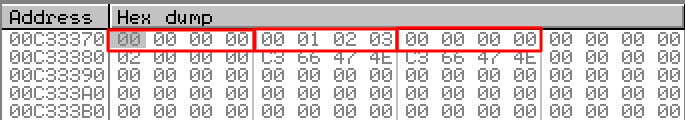
\includegraphics[scale=\NormalScale]{patterns/13_arrays/5_multidimensional/olly_2D_1.png}
\caption{\olly: array is filled}
\end{figure}

\subsubsection{Column filling example}
\myindex{\olly}

Let's fill the third column with values: 0..2:

\lstinputlisting[caption=Column filling example]{patterns/13_arrays/5_multidimensional/two2_EN.c}

The three rows are also marked in red here. 

We see that in each row, at third position these values are written: 0, 1 and 2.

\begin{figure}[H]
\centering
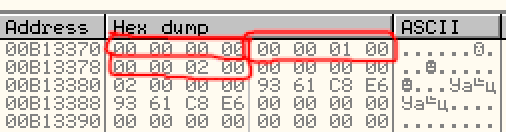
\includegraphics[scale=\NormalScale]{patterns/13_arrays/5_multidimensional/olly_2D_2.png}
\caption{\olly: array is filled}
\end{figure}


\subsubsection{Access two-dimensional array as one-dimensional}

We can be easily assured that it's possible to access a two-dimensional array as one-dimensional array in at least two ways:

\lstinputlisting{patterns/13_arrays/5_multidimensional/2D_as_1D_EN.c}

Compile and run it: it shows correct values.

What MSVC 2013 did is fascinating, all three routines are just the same!

\lstinputlisting[caption=\Optimizing MSVC 2013 x64]{patterns/13_arrays/5_multidimensional/2D_as_1D_MSVC_2013_Ox_x64_EN.asm}

GCC also generates equivalent routines, but slightly different:

\lstinputlisting[caption=\Optimizing GCC 4.9 x64]{patterns/13_arrays/5_multidimensional/2D_as_1D_GCC49_x64_O3_EN.s}


\subsubsection{Three-dimensional array example}

It's the same for multidimensional arrays.

Now we are going to work with an array of type \Tint: each element requires 4 bytes in memory.

Let's see:

\lstinputlisting[caption=simple example]{patterns/13_arrays/5_multidimensional/multi.c}

\myparagraph{x86}

We get (MSVC 2010):

\lstinputlisting[caption=MSVC 2010]{patterns/13_arrays/5_multidimensional/multi_msvc_EN.asm}

Nothing special. For index calculation, three input arguments are used 
in the formula $address=600 \cdot 4 \cdot x + 30 \cdot 4 \cdot y + 4z$, to represent the array as multidimensional.
Do not forget that the \Tint type is 32-bit (4 bytes),
so all coefficients must be multiplied by 4.

\lstinputlisting[caption=GCC 4.4.1]{patterns/13_arrays/5_multidimensional/multi_gcc_EN.asm}

The GCC compiler does it differently.

For one of the operations in the calculation ($30y$), GCC produces code without multiplication instructions.
This is how it done: 
$(y+y) \ll 4 - (y+y) = (2y) \ll 4 - 2y = 2 \cdot 16 \cdot y - 2y = 32y - 2y = 30y$. 
Thus, for the $30y$ calculation, only one addition operation,
one bitwise shift operation and one subtraction operation are used.
This works faster.

\myparagraph{ARM + \NonOptimizingXcodeIV (\ThumbMode)}

\lstinputlisting[caption=\NonOptimizingXcodeIV (\ThumbMode)]{patterns/13_arrays/5_multidimensional/multi_Xcode_thumb_O0_EN.asm}

\NonOptimizing LLVM saves all variables in local stack, which is redundant.

The address of the array element is calculated by the formula we already saw.

\myparagraph{ARM + \OptimizingXcodeIV (\ThumbMode)}

\lstinputlisting[caption=\OptimizingXcodeIV (\ThumbMode)]{patterns/13_arrays/5_multidimensional/multi_Xcode_thumb_O3_EN.asm}

The tricks for replacing multiplication by shift, addition and subtraction which we already saw
are also present here.

\myindex{ARM!\Instructions!RSB}
\myindex{ARM!\Instructions!SUB}
Here we also see a new instruction for us: \RSB (\IT{Reverse Subtract}).

It works just as \SUB, but it swaps its operands with each other before execution.
Why?
\myindex{ARM!Optional operators!LSL}
\SUB and \RSB  are instructions, to the second operand of which shift coefficient may be applied: (\INS{LSL\#4}). 

But this coefficient can be applied only to second operand.

That's fine for commutative operations like addition or multiplication 
(operands may be swapped there without changing the result).

But subtraction is a non-commutative operation, so \RSB exist for these cases.

\myindex{ARM!\Instructions!LDR.W}
The \INS{LDR.W R9, [R9]} instruction works like \LEA~(\myref{sec:LEA})

in x86, but it does nothing here, it is redundant.
Apparently, the compiler did not optimize it out.

\myparagraph{MIPS}

\myindex{MIPS!Global Pointer}
My example is tiny, so the GCC compiler decided to put the $a$ array into the 64KiB area 
addressable by the Global Pointer.

\lstinputlisting[caption=\Optimizing GCC 4.4.5 (IDA)]{patterns/13_arrays/5_multidimensional/multi_MIPS_O3_IDA_EN.lst}



\subsubsection{More examples}

The computer screen is represented as a 2D array, but the video-buffer is a linear 1D array. 
We talk about it here: \myref{Mandelbrot_demo}.

Another example in this book is Minesweeper game: it's field is also two-dimensional array: \ref{minesweeper_winxp}.

}
\RU{\section{Многомерные массивы}

Внутри многомерный массив выглядит так же как и линейный.

Ведь память компьютера линейная, это одномерный массив.
Но для удобства этот одномерный массив легко представить как многомерный.

К примеру, вот как элементы массива 3x4 расположены в одномерном массиве из 12 ячеек:

% TODO FIXME not clear. First, horizontal would be better. Second, why two columns?
% I'd first show 3x4 with numbered elements (e.g. 32-bit ints) in colored lines,
% then linear with the same numbered elements (and colored blocks)
% then linear with addresses (offsets) - assuming let say 32-bit ints.
\begin{table}[H]
\centering
\begin{tabular}{ | l | l | }
\hline
Смещение в памяти & элемент массива \\
\hline
0 & [0][0] \\
\hline
1 & [0][1] \\
\hline
2 & [0][2] \\
\hline
3 & [0][3] \\
\hline
4 & [1][0] \\
\hline
5 & [1][1] \\
\hline
6 & [1][2] \\
\hline
7 & [1][3] \\
\hline
8 & [2][0] \\
\hline
9 & [2][1] \\
\hline
10 & [2][2] \\
\hline
11 & [2][3] \\
\hline
\end{tabular}
\caption{Двухмерный массив представляется в памяти как одномерный}
\end{table}

Вот по каким адресам в памяти располагается каждая ячейка двухмерного массива 3*4:

\begin{table}[H]
\centering
\begin{tabular}{ | l | l | l | l | }
\hline                        
0 & 1 & 2 & 3 \\
\hline  
4 & 5 & 6 & 7 \\
\hline  
8 & 9 & 10 & 11 \\
\hline  
\end{tabular}
\caption{Адреса в памяти каждой ячейки двухмерного массива}
\end{table}

\myindex{row-major order}
Чтобы вычислить адрес нужного элемента, сначала умножаем первый индекс (строку) на 4 (ширину массива), 
затем прибавляем второй индекс (столбец).

Это называется \IT{row-major order}, 
и такой способ представления массивов и матриц используется по крайней мере в \CCpp и Python. 
Термин \IT{row-major order} означает по-русски примерно следующее: \q{сначала записываем элементы первой строки, затем второй,~\dots~и~элементы последней 
строки в самом конце}.

\myindex{column-major order}
\myindex{Фортран}
Другой способ представления называется \IT{column-major order} (индексы массива используются в обратном порядке) 
и это используется по крайней мере в Фортране, MATLAB и R. 
Термин \IT{column-major order} означает по-русски
следующее: \q{сначала записываем элементы первого столбца, затем второго,~\dots~и~элементы последнего столбца
в самом конце}.

Какой из способов лучше?
В терминах производительности и кэш-памяти, лучший метод организации данных это тот,
при котором к данным обращаются последовательно.

Так что если ваша функция обращается к данным построчно, то \IT{row-major order} лучше,
и наоборот.

% subsections
\subsubsection{Пример с двумерным массивов}

Мы будем работать с массивом типа \Tchar. Это значит, что каждый элемент требует
только одного байта в памяти.

\myparagraph{Пример с заполнением строки}
\myindex{\olly}

Заполняем вторую строку значениями 0..3:

\lstinputlisting[caption=Пример с заполнением строки]{patterns/13_arrays/5_multidimensional/two1_RU.c}

Все три строки обведены красным. 
Видно, что во второй теперь имеются байты 0, 1, 2 и 3:

\begin{figure}[H]
\centering
\myincludegraphics{patterns/13_arrays/5_multidimensional/olly_2D_1.png}
\caption{\olly: массив заполнен}
\end{figure}

\myparagraph{Пример с заполнением столбца}
\myindex{\olly}

Заполняем третий столбец значениями 0..2:

\lstinputlisting[caption=Пример с заполнением столбца]{patterns/13_arrays/5_multidimensional/two2_RU.c}

Здесь также обведены красным три строки. 
Видно, что в каждой строке, на третьей позиции, теперь записаны 0, 1 и 2.

\begin{figure}[H]
\centering
\myincludegraphics{patterns/13_arrays/5_multidimensional/olly_2D_2.png}
\caption{\olly: массив заполнен}
\end{figure}

\subsectionold{Работа с двухмерным массивом как с одномерным}

Мы можем легко убедиться, что можно работать с двухмерным массивом как с одномерным,
используя по крайней мере два метода:

\lstinputlisting{patterns/13_arrays/5_multidimensional/2D_as_1D_RU.c}

Компилируете и запускаете: мы увидим корректные значения.

Очарователен результат работы MSVC 2013~--- все три процедуры одинаковые!

\lstinputlisting[caption=\Optimizing MSVC 2013 x64]{patterns/13_arrays/5_multidimensional/2D_as_1D_MSVC_2013_Ox_x64_RU.asm}

GCC сгенерировал практически одинаковые процедуры:

\lstinputlisting[caption=\Optimizing GCC 4.9 x64]{patterns/13_arrays/5_multidimensional/2D_as_1D_GCC49_x64_O3_RU.s}


\subsection{Пример с трехмерным массивом}

То же самое и для многомерных массивов.
На этот раз будем работать с массивом типа \Tint: каждый элемент требует 4 байта в памяти.

Попробуем:

\lstinputlisting[caption=простой пример]{patterns/13_arrays/5_multidimensional/multi.c}

\subsubsection{x86}

В итоге (MSVC 2010):

\lstinputlisting[caption=MSVC 2010]{patterns/13_arrays/5_multidimensional/multi_msvc_RU.asm}

В принципе, ничего удивительного. В \TT{insert()} для вычисления адреса нужного элемента массива 
три входных аргумента перемножаются по формуле $address=600 \cdot 4 \cdot x + 30 \cdot 4 \cdot y + 4z$, 
чтобы представить массив трехмерным.
Не забывайте также, что тип \Tint 32-битный (4 байта), поэтому все коэффициенты нужно умножить на 4.

\lstinputlisting[caption=GCC 4.4.1]{patterns/13_arrays/5_multidimensional/multi_gcc_RU.asm}

Компилятор GCC решил всё сделать немного иначе.
Для вычисления одной из операций ($30y$), GCC создал код, где нет самой операции умножения.

Происходит это так: 
$(y+y) \ll 4 - (y+y) = (2y) \ll 4 - 2y = 2 \cdot 16 \cdot y - 2y = 32y - 2y = 30y$. 
Таким образом, для вычисления $30y$ используется только операция сложения, 
операция битового сдвига и операция вычитания.
Это работает быстрее.

\subsubsection{ARM + \NonOptimizingXcodeIV (\ThumbMode)}

\lstinputlisting[caption=\NonOptimizingXcodeIV (\ThumbMode)]{patterns/13_arrays/5_multidimensional/multi_Xcode_thumb_O0_RU.asm}

\NonOptimizing LLVM сохраняет все переменные в локальном стеке, хотя это и избыточно.

Адрес элемента массива вычисляется по уже рассмотренной формуле.

\subsubsection{ARM + \OptimizingXcodeIV (\ThumbMode)}

\lstinputlisting[caption=\OptimizingXcodeIV (\ThumbMode)]{patterns/13_arrays/5_multidimensional/multi_Xcode_thumb_O3_RU.asm}

Тут используются уже описанные трюки для замены умножения на операции сдвига, сложения и вычитания.

\myindex{ARM!\Instructions!RSB}
\myindex{ARM!\Instructions!SUB}
Также мы видим новую для себя инструкцию \RSB (\IT{Reverse Subtract}).
Она работает так же, как и \SUB, только меняет операнды местами.

Зачем?
\myindex{ARM!Optional operators!LSL}
\SUB и \RSB это те инструкции, ко второму операнду которых можно применить коэффициент сдвига, как мы видим и здесь: (\INS{LSL\#4}). 
Но этот коэффициент можно применить только ко второму операнду.

Для коммутативных операций, таких как сложение или умножение, 
операнды можно менять местами и это не влияет на результат.

Но вычитание~--- операция некоммутативная, так что для этих случаев существует инструкция \RSB.

\myindex{ARM!\Instructions!LDR.W}
Инструкция \INS{LDR.W R9, [R9]} работает как \LEA~(\myref{sec:LEA}) в x86, и здесь она ничего не делает, она избыточна.

Вероятно, компилятор не оптимизировал её.

\subsubsection{MIPS}

\myindex{MIPS!Global Pointer}

Мой пример такой крошечный, что компилятор GCC решил разместить массив $a$ в 64KiB-области,
адресуемой при помощи Global Pointer.

\lstinputlisting[caption=\Optimizing GCC 4.4.5 (IDA)]{patterns/13_arrays/5_multidimensional/multi_MIPS_O3_IDA_RU.lst}



\subsection{Ещё примеры}

Компьютерный экран представляет собой двумерный массив, но видеобуфер это линейный
одномерный массив. 
Мы рассматриваем это здесь: \myref{Mandelbrot_demo}.

Еще один пример в этой книге это игра ``Сапер'': её поле это тоже двухмерный массив: \ref{minesweeper_winxp}.

}
\EN{\section{Pack of strings as a two-dimensional array}

Let's revisit the function that returns the name of a month: \lstref{get_month1}.

As you see, at least one memory load operation is needed to prepare a pointer to the string
that's the month's name.

Is it possible to get rid of this memory load operation?

In fact yes, if you represent the list of strings as a two-dimensional array:

\lstinputlisting{patterns/13_arrays/55_month_2D/month2_EN.c}

Here is what we've get:

\lstinputlisting[caption=\Optimizing MSVC 2013 x64]{patterns/13_arrays/55_month_2D/MSVC2013_x64_Ox_EN.asm}

There are no memory accesses at all.

All this function does is to calculate a point at which the first character of the name of the month is: 
$pointer\_to\_the\_table + month * 10$.

There are also two \LEA instructions, which effectively work as several \MUL and \MOV instructions.

The width of the array is 10 bytes. 

Indeed, the longest string here---\q{September}---is 9 bytes, and plus the terminating zero is 10 bytes.

The rest of the month names are padded by zero bytes, so they all occupy the same space (10 bytes).

Thus, our function works even faster, because all string start at an address which can be
calculated easily.

\Optimizing GCC 4.9 can do it even shorter:

\begin{lstlisting}[caption=\Optimizing GCC 4.9 x64]
	movsx	rdi, edi
	lea	rax, [rdi+rdi*4]
	lea	rax, month2[rax+rax]
	ret
\end{lstlisting}

\LEA is also used here for multiplication by 10.

Non-optimizing compilers do multiplication differently.

\lstinputlisting[caption=\NonOptimizing GCC 4.9 x64]{patterns/13_arrays/55_month_2D/x64_GCC49_O0_EN.asm}

\NonOptimizing MSVC just uses \IMUL instruction:
\myindex{x86!\Instructions!IMUL}

\lstinputlisting[caption=\NonOptimizing MSVC 2013 x64]{patterns/13_arrays/55_month_2D/MSVC2013_x64_EN.asm}

\myindex{\CompilerAnomaly}
\label{MSVC2013_anomaly}

But one thing is weird here: why add multiplication by zero and adding zero to the final result?

This looks like a compiler code generator quirk, which wasn't caught by the compiler's tests
(the resulting code works correctly, after all).
% класс!
%
We intentionally consider such pieces of code so the reader would understand, 
that sometimes one shouldn't puzzle over such compiler artifacts.

\subsection{32-bit ARM}

\Optimizing Keil 
for Thumb mode uses the multiplication instruction \INS{MULS}:

\lstinputlisting[caption=\OptimizingKeilVI (\ThumbMode)]{patterns/13_arrays/55_month_2D/Keil_O3_thumb_EN.asm}

\Optimizing Keil for ARM mode uses add and shift operations:

\lstinputlisting[caption=\OptimizingKeilVI (\ARMMode)]{patterns/13_arrays/55_month_2D/Keil_O3_ARM_EN.asm}

\subsection{ARM64}

\lstinputlisting[caption=\Optimizing GCC 4.9 ARM64]{patterns/13_arrays/55_month_2D/GCC49_ARM64_EN.asm}

\myindex{ARM!\Instructions!SXTW}
\myindex{ARM!\Instructions!ADRP/ADD pair}

\INS{SXTW} is used for sign-extension and promoting input 32-bit value into a 64-bit one and storing it in X0.

\ADRP/\ADD pair is used for loading the address of the table.

The \ADD instructions also has a \LSL suffix, which helps with multiplications.

\subsection{MIPS}
\lstinputlisting[caption=\Optimizing GCC 4.4.5 (IDA)]{patterns/13_arrays/55_month_2D/MIPS_O3_IDA_EN.lst}

\subsection{\Conclusion{}}

This is a bit old-school technique to store text strings.

You may find a lot of it in \oracle, for example.

It's hard to say if it's worth doing on modern computers.

Nevertheless, it was a good example of arrays, so it was added to this book.

}
\RU{\section{Набор строк как двухмерный массив}

Снова вернемся к примеру, который возвращает название месяца: \lstref{get_month1}.
Как видно, нужна как минимум одна операция загрузки из памяти для подготовки указателя на строку,
состоящую из имени месяца.

Возможно ли избавиться от операции загрузки из памяти?

Да, если представить список строк как двумерный массив:

\lstinputlisting{patterns/13_arrays/55_month_2D/month2_RU.c}

Вот что получаем:

\lstinputlisting[caption=\Optimizing MSVC 2013 x64]{patterns/13_arrays/55_month_2D/MSVC2013_x64_Ox_RU.asm}

Здесь нет обращений к памяти вообще.
Эта функция только вычисляет место, где находится первый символ названия месяца:
 
$pointer\_to\_the\_table + month * 10$.
Там также две инструкции \LEA, которые работают как несколько инструкций \MUL и \MOV.

Ширина массива~--- 10 байт. 
Действительно, самая длинная строка это \q{September} (9 байт) плюс оконечивающий ноль, получается 10 байт.

Остальные названия месяцев дополнены нулевыми байтами, чтобы они занимали столько же места (10 байт).

Таким образом, наша функция и работает быстрее, потому что все строки начинаются с тех адресов, 
которые легко вычислить.

\Optimizing GCC 4.9 может ещё короче:

\begin{lstlisting}[caption=\Optimizing GCC 4.9 x64]
	movsx	rdi, edi
	lea	rax, [rdi+rdi*4]
	lea	rax, month2[rax+rax]
	ret
\end{lstlisting}

\LEA здесь также используется для умножения на 10.

Неоптимизирующие компиляторы делают умножение по-разному.

\lstinputlisting[caption=\NonOptimizing GCC 4.9 x64]{patterns/13_arrays/55_month_2D/x64_GCC49_O0_RU.asm}

\NonOptimizing MSVC просто использует инструкцию \IMUL:
\myindex{x86!\Instructions!IMUL}

\lstinputlisting[caption=\NonOptimizing MSVC 2013 x64]{patterns/13_arrays/55_month_2D/MSVC2013_x64_RU.asm}

\myindex{\CompilerAnomaly}
\label{MSVC2013_anomaly}
Но вот что странно: зачем добавлять умножение на ноль и добавлять ноль к конечному результату?

Это выглядит как странность кодегенератора компилятора, который не был покрыт тестами
компилятора. Но так или иначе, итоговый код работает корректно.
% класс! ЩИТО?
Мы сознательно рассматриваем такие фрагменты кода, чтобы читатель понимал, что иногда не нужно
ломать себе голову над подобными артефактами компиляторов.

\subsection{32-bit ARM}

\Optimizing Keil для режима Thumb использует инструкцию умножения \INS{MULS}:

\lstinputlisting[caption=\OptimizingKeilVI (\ThumbMode)]{patterns/13_arrays/55_month_2D/Keil_O3_thumb_RU.asm}

\Optimizing Keil для режима ARM использует операции сложения и сдвига:

\lstinputlisting[caption=\OptimizingKeilVI (\ARMMode)]{patterns/13_arrays/55_month_2D/Keil_O3_ARM_RU.asm}

\subsection{ARM64}

\lstinputlisting[caption=\Optimizing GCC 4.9 ARM64]{patterns/13_arrays/55_month_2D/GCC49_ARM64_RU.asm}

\myindex{ARM!\Instructions!SXTW}
\myindex{ARM!\Instructions!ADRP/ADD pair}
\INS{SXTW} используется для знакового расширения и расширения
входного 32-битного значения в 64-битное и сохранения его в X0.

Пара \ADRP/\ADD используется для загрузки адреса таблицы.

У инструкции \ADD также есть суффикс \LSL, что помогает с умножением.

\subsection{MIPS}
\lstinputlisting[caption=\Optimizing GCC 4.4.5 (IDA)]{patterns/13_arrays/55_month_2D/MIPS_O3_IDA_RU.lst}

\subsection{\Conclusion{}}

Это немного старинная техника для хранения текстовых строк.

Много такого можно найти в \oracle, например.

Трудно сказать, стоит ли оно того на современных компьютерах.

Так или иначе, это был хороший пример массивов, поэтому он был добавлен в эту книгу.

}
\subsection{\Conclusion{}}

\RU{Массив это просто набор значений в памяти, расположенных рядом друг с другом.}
\EN{An array is a pack of values in memory located adjacently.}
\RU{Это справедливо для любых типов элементов, включая структуры.}
\EN{It's true for any element type, including structures.}
\RU{Доступ к определенному элементу массива это просто вычисление его адреса.}
\EN{Access to a specific array element is just a calculation of its address.}

\section{\Exercises}

\subsection{\Exercise \#1}
% matrix addition
\label{exercise_array_1}

\WhatThisCodeDoes\

\lstinputlisting[caption=MSVC 2010 + \TT{/O1}]{patterns/13_arrays/exercises/1_msvc.asm}

(/O1: \RU{оптимизация по размеру кода}\EN{minimize space}).

\lstinputlisting[caption=Keil 5.03 (\ARMMode) + \Othree]{patterns/13_arrays/exercises/1_ARM.s}

\lstinputlisting[caption=Keil 5.03 (\ThumbMode) + \Othree]{patterns/13_arrays/exercises/1_thumb.s}

\Answer\: \ref{exercise_solutions_arrays_1}.

\subsection{\Exercise \#2}
% matrix multiplication
\label{exercise_array_2}

\WhatThisCodeDoes\

\lstinputlisting[caption=MSVC 2010 + \TT{/O1}]{patterns/13_arrays/exercises/2_msvc.asm}

(/O1: \RU{оптимизация по размеру кода}\EN{minimize space}).

\lstinputlisting[caption=Keil 5.03 (\ARMMode) + \Othree]{patterns/13_arrays/exercises/2_ARM.s}

\lstinputlisting[caption=Keil 5.03 (\ThumbMode) + \Othree]{patterns/13_arrays/exercises/2_thumb.s}

\Answer\: \ref{exercise_solutions_arrays_2}.

\subsection{\Exercise \#3}
\label{exercise_array_3}

\WhatThisCodeDoes\

\EN{Try to determine array size, at least partially.}
\RU{Попробуйте определить размеры массива, хотя бы частично.}

\begin{lstlisting}[caption=MSVC 2010 /Ox]
_array$ = 8
_x$ = 12
_y$ = 16
_f	PROC
	mov	eax, DWORD PTR _x$[esp-4]
	mov	edx, DWORD PTR _y$[esp-4]
	mov	ecx, eax
	shl	ecx, 4
	sub	ecx, eax
	lea	eax, DWORD PTR [edx+ecx*8]
	mov	ecx, DWORD PTR _array$[esp-4]
	fld	QWORD PTR [ecx+eax*8]
	ret	0
_f	ENDP
\end{lstlisting}

\begin{lstlisting}[caption=Keil 5.03 (\ARMMode)]
f PROC
        RSB      r1,r1,r1,LSL #4
        ADD      r0,r0,r1,LSL #6
        ADD      r1,r0,r2,LSL #3
        LDM      r1,{r0,r1}
        BX       lr
        ENDP
\end{lstlisting}

\begin{lstlisting}[caption=Keil 5.03 (\ThumbMode)]
f PROC
        MOVS     r3,#0xf
        LSLS     r3,r3,#6
        MULS     r1,r3,r1
        ADDS     r0,r1,r0
        LSLS     r1,r2,#3
        ADDS     r1,r0,r1
        LDM      r1,{r0,r1}
        BX       lr
        ENDP
\end{lstlisting}

\Answer\: \ref{exercise_solutions_arrays_3}

\subsection{\Exercise \#4}
\label{exercise_array_4}

\WhatThisCodeDoes\

\EN{Try to determine array size, at least partially.}
\RU{Попробуйте определить размеры массива, хотя бы частично.}

\begin{lstlisting}[caption=MSVC 2010 /Ox]
_array$ = 8	
_x$ = 12	
_y$ = 16	
_z$ = 20	
_f	PROC
	mov	eax, DWORD PTR _x$[esp-4]
	mov	edx, DWORD PTR _y$[esp-4]
	mov	ecx, eax
	shl	ecx, 4
	sub	ecx, eax
	lea	eax, DWORD PTR [edx+ecx*4]
	mov	ecx, DWORD PTR _array$[esp-4]
	lea	eax, DWORD PTR [eax+eax*4]
	shl	eax, 4
	add	eax, DWORD PTR _z$[esp-4]
	mov	eax, DWORD PTR [ecx+eax*4]
	ret	0
_f	ENDP
\end{lstlisting}

\begin{lstlisting}[caption=Keil 5.03 (\ARMMode)]
f PROC
        RSB      r1,r1,r1,LSL #4
        ADD      r1,r1,r1,LSL #2
        ADD      r0,r0,r1,LSL #8
        ADD      r1,r2,r2,LSL #2
        ADD      r0,r0,r1,LSL #6
        LDR      r0,[r0,r3,LSL #2]
        BX       lr
        ENDP
\end{lstlisting}

\begin{lstlisting}[caption=Keil 5.03 (\ThumbMode)]
f PROC
        PUSH     {r4,lr}
        MOVS     r4,#0x4b
        LSLS     r4,r4,#8
        MULS     r1,r4,r1
        ADDS     r0,r1,r0
        MOVS     r1,#0xff
        ADDS     r1,r1,#0x41
        MULS     r2,r1,r2
        ADDS     r0,r0,r2
        LSLS     r1,r3,#2
        LDR      r0,[r0,r1]
        POP      {r4,pc}
        ENDP
\end{lstlisting}

\Answer\: \ref{exercise_solutions_arrays_4}

\subsection{\Exercise \#5}
\label{exercise_array_5}

\WhatThisCodeDoes\

\begin{lstlisting}[caption=MSVC 2012 /Ox /GS-]
COMM	_tbl:DWORD:064H

tv759 = -4	; size = 4
_main	PROC
	push	ecx
	push	ebx
	push	ebp
	push	esi
	xor	edx, edx
	push	edi
	xor	esi, esi
	xor	edi, edi
	xor	ebx, ebx
	xor	ebp, ebp
	mov	DWORD PTR tv759[esp+20], edx
	mov	eax, OFFSET _tbl+4
	npad	8
$LL6@main:
	lea	ecx, DWORD PTR [edx+edx]
	mov	DWORD PTR [eax+4], ecx
	mov	ecx, DWORD PTR tv759[esp+20]
	add	DWORD PTR tv759[esp+20], 3
	mov	DWORD PTR [eax+8], ecx
	lea	ecx, DWORD PTR [edx*4]
	mov	DWORD PTR [eax+12], ecx
	lea	ecx, DWORD PTR [edx*8]
	mov	DWORD PTR [eax], edx
	mov	DWORD PTR [eax+16], ebp
	mov	DWORD PTR [eax+20], ebx
	mov	DWORD PTR [eax+24], edi
	mov	DWORD PTR [eax+32], esi
	mov	DWORD PTR [eax-4], 0
	mov	DWORD PTR [eax+28], ecx
	add	eax, 40
	inc	edx
	add	ebp, 5
	add	ebx, 6
	add	edi, 7
	add	esi, 9
	cmp	eax, OFFSET _tbl+404
	jl	SHORT $LL6@main
	pop	edi
	pop	esi
	pop	ebp
	xor	eax, eax
	pop	ebx
	pop	ecx
	ret	0
_main	ENDP
\end{lstlisting}

\begin{lstlisting}[caption=Keil 5.03 (\ARMMode)]
main PROC
        LDR      r12,|L0.60|
        MOV      r1,#0
|L0.8|
        ADD      r2,r1,r1,LSL #2
        MOV      r0,#0
        ADD      r2,r12,r2,LSL #3
|L0.20|
        MUL      r3,r1,r0
        STR      r3,[r2,r0,LSL #2]
        ADD      r0,r0,#1
        CMP      r0,#0xa
        BLT      |L0.20|
        ADD      r1,r1,#1
        CMP      r1,#0xa
        MOVGE    r0,#0
        BLT      |L0.8|
        BX       lr
        ENDP

|L0.60|
        DCD      ||.bss||

        AREA ||.bss||, DATA, NOINIT, ALIGN=2

tbl
        %        400
\end{lstlisting}

\begin{lstlisting}[caption=Keil 5.03 (\ThumbMode)]
main PROC
        PUSH     {r4,r5,lr}
        LDR      r4,|L0.40|
        MOVS     r1,#0
|L0.6|
        MOVS     r2,#0x28
        MULS     r2,r1,r2
        MOVS     r0,#0
        ADDS     r3,r2,r4
|L0.14|
        MOVS     r2,r1
        MULS     r2,r0,r2
        LSLS     r5,r0,#2
        ADDS     r0,r0,#1
        CMP      r0,#0xa
        STR      r2,[r3,r5]
        BLT      |L0.14|
        ADDS     r1,r1,#1
        CMP      r1,#0xa
        BLT      |L0.6|
        MOVS     r0,#0
        POP      {r4,r5,pc}
        ENDP

        DCW      0x0000
|L0.40|
        DCD      ||.bss||

        AREA ||.bss||, DATA, NOINIT, ALIGN=2

tbl
        %        400
\end{lstlisting}

\Answer\: \ref{exercise_solutions_arrays_5}

